%!TEX root=qsic2014.tex
% mainfile: qsic2014.tex

\begin{figure}[!t]
\centering
\captionsetup{justification=centering}
  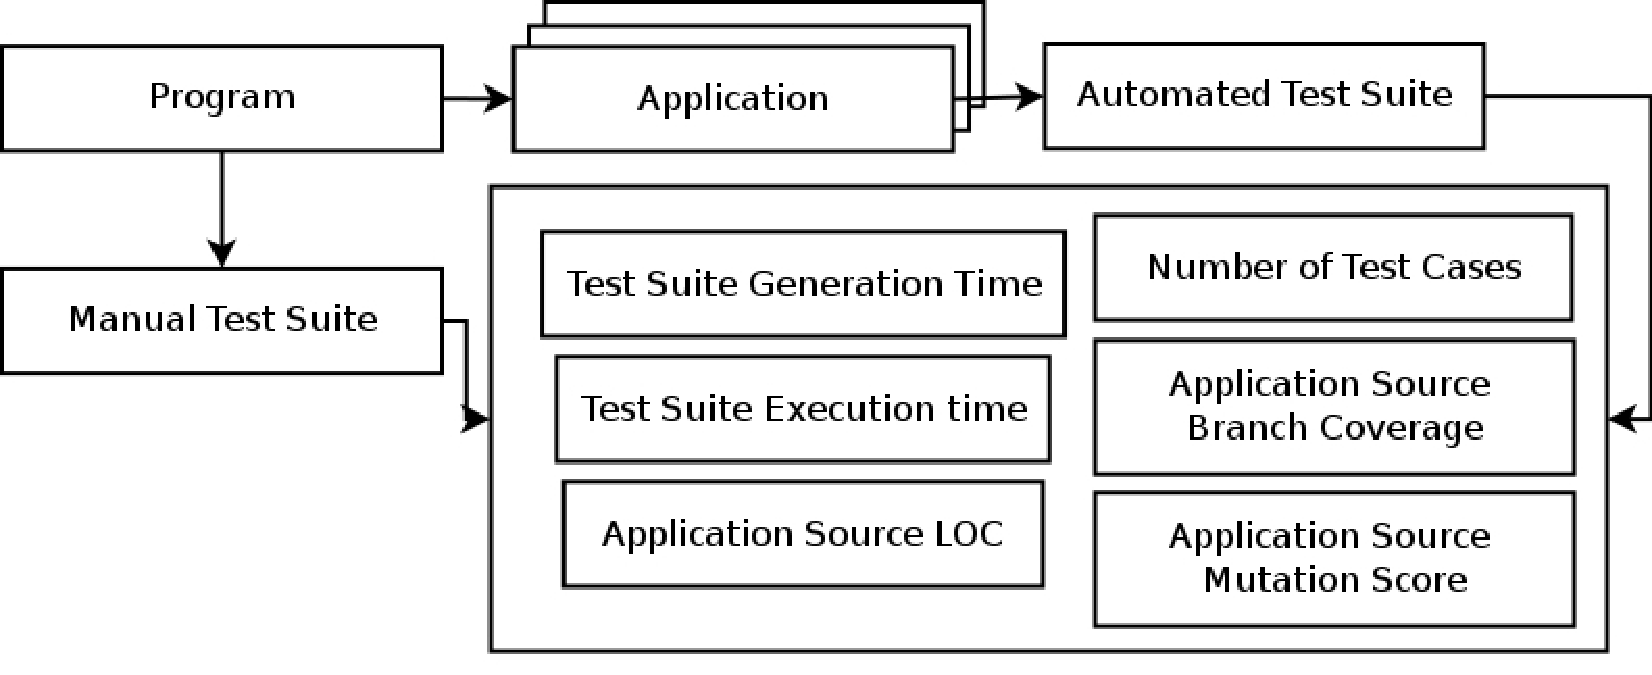
\includegraphics[width=\linewidth]{proccess_diagram.pdf}
    \caption{Evaluation Process}
  \label{fig:process_diagram}
\end{figure}

\section{Empirical Evaluation}
\label{sec:evaluation}
Given the many different techniques for generating test suites, the primary goal of this paper's empirical study is to compare the quality and complexity of the resulting test suites.  We implemented the empirical evaluation approach as shown in Figure~\ref{fig:process_diagram}.  As can be seen in the figure, existing programs are fed into automatic test suite generators to create executable test suites.  These test suites are then compared to the programs' associated, manually written test suites based on six metrics.   

The goals of the experiments are as follows:
\squishlist
\item Determine the time of automated test case generation along with the size and time of execution of the test suites
\item Compare the test suites, automatically generated and manually written, compared to the case studies' source code
\item Analyze the quality of these test suites based on branch coverage and fault-based mutation scores
%\item Do automated or manual test suites create enough quality tests for more complex applications?
%\item What is the difference in quality between automated test suite generators and manually written test suites?
%\item Does the size of an application  effect the branch coverage and mutation scores of automated and manually generated test suites?
%\item Are branch coverage and mutation scores always the best indicators that a test suite reduces cost and effort?
\squishend

\subsection{Experiment Design and Metrics}
All experiments were performed on GNU/Linux workstations with kernel 3.2.0-44, a 2 GHz Intel Corporation Xeon E5/Core i7 processor and  15.6 GB of main memory. 
\begin{table}[!t]
\centering
\caption{Benchmark Programs and their Properties}
\label{tbl:program_table}
%\resizebox{\columnwidth}{!}{%
\begin{tabular}{|l|c|c|}
\hline
\textbf{Program} & \textbf{LOC} &\textbf{Cyclomatic Complexity} \\ \hline
Netweaver                              & 17953                              & 2.82                                                \\ \hline
Inspirento                             & 1769                               & 1.76                                                \\ \hline
Jsecurity                              & 9470                               & 2.05                                                \\ \hline
Saxpath                                & 1441                               & 2.10                                                \\ \hline
Jni-inchi                              & 783                                & 2.05                                                \\ \hline
Xisemele                               & 1399                               & 1.29                                                \\ \hline
Diebierse                              & 1539                               & 1.74                                                \\ \hline
Lagoon                                 & 6060                               & 3.52                                                \\ \hline
Lavalamp                               & 1039                               & 1.50                                                \\ \hline
Jnfe                                   & 1294                               & 1.38                                                \\ \hline
\end{tabular}
%}
\end{table}

\noindent \textbf{Case Study Applications:}  

Ten programs were identified from the SF110 code suite~\cite{fraser:2012}.  The case study applications were selected due to their size, the existence of associated manually developed JUnit test cases, and their use in tuning \textsc{EvoSuite} parameters for mutation and test generation, one of our test suite generation tools.  Table~\ref{tbl:program_table} provides a list of the selected SF110 programs with their respective lines of code (LOC) and average cyclomatic complexity per method.  LOC and cyclomatic complexity were measured using JavaNCSS~\cite{leejavancss}.  

\begin{figure*}[!t]
\centering
  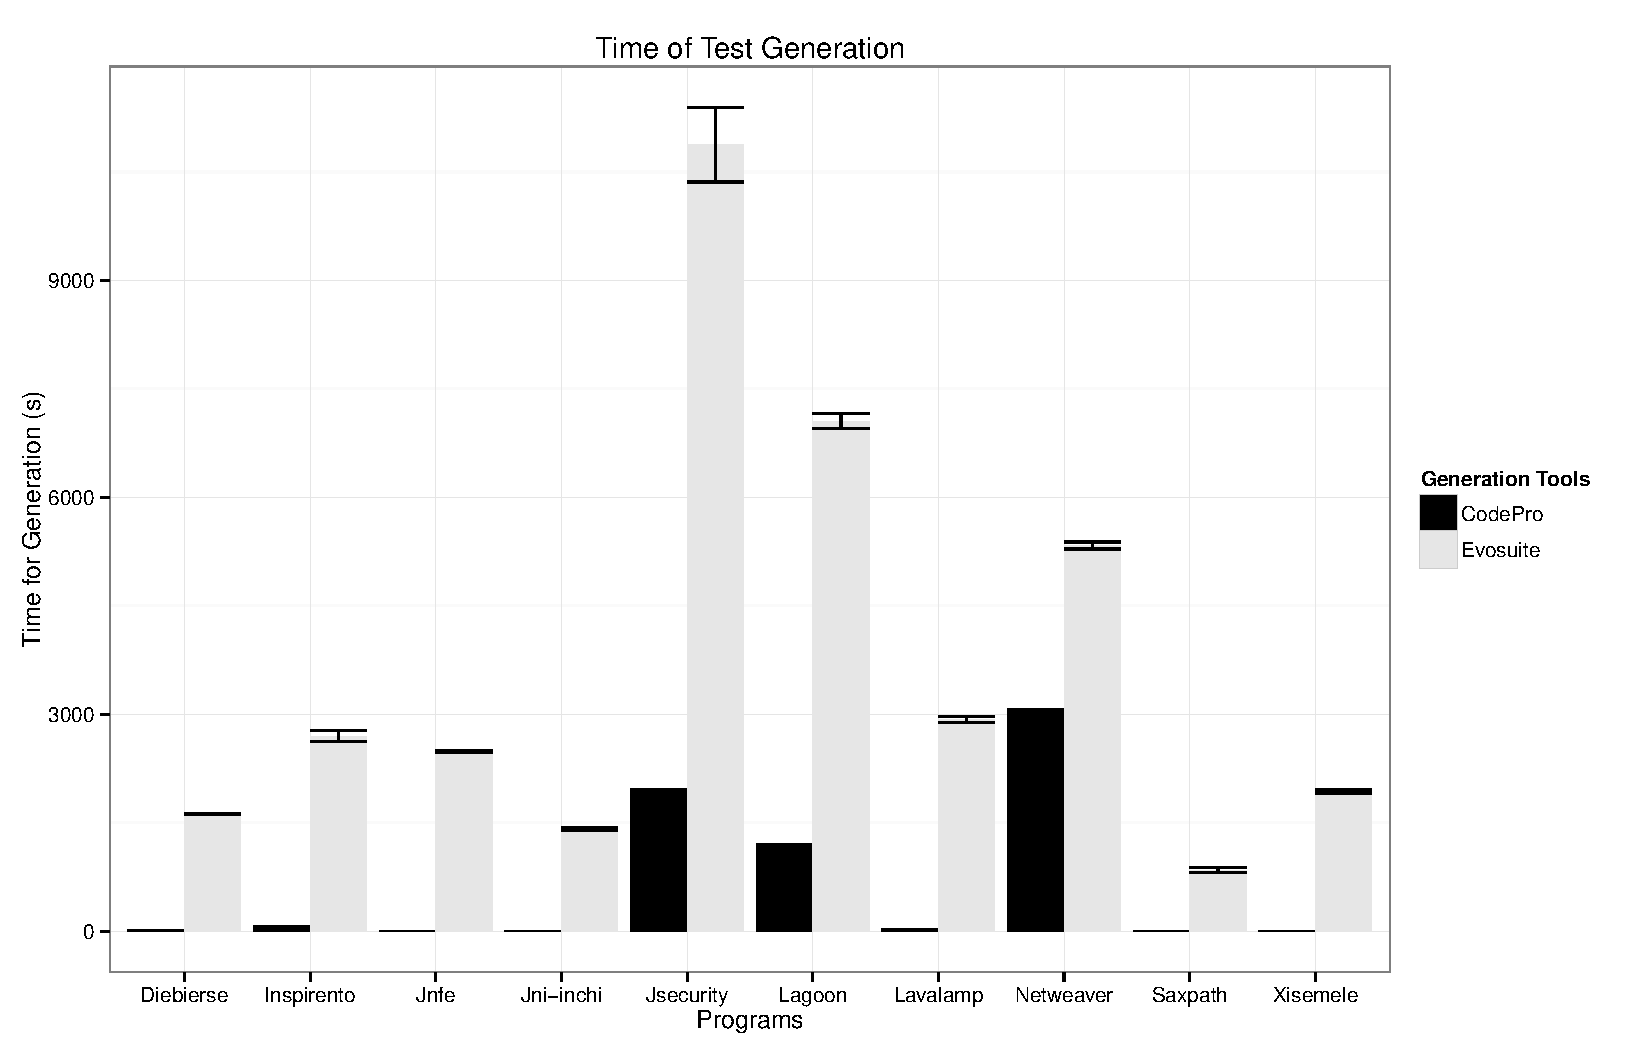
\includegraphics[scale=0.5]{RGraphs/TimeOfGeneration.pdf}
    \caption{Time to Generate Test Suites.}
  \label{fig:TimeGen}
\end{figure*}

%Can cut from this paragraph
Netweaver is the largest program under consideration with nearly 18K lines of code.  Netweaver has an average Cyclomatic Complexity ($CC$) of 2.82 across all methods, which implies that for a specific method $M$, 1) $CC_M$ is an upper bound for the number of test cases that are necessary to achieve a complete branch coverage within the method $M$, and 2) $CC_M$ is a lower bound for the number of paths through the control flow graph. Assuming each test case takes one path, the number of cases needed to achieve path coverage is equal to the number of paths that can actually be taken, ignoring infeasible paths.  The smallest program, Jni-inchi has 783 lines of code with an average cyclomatic complexity of 2.05.  

\begin{figure*}[!t]
\centering
  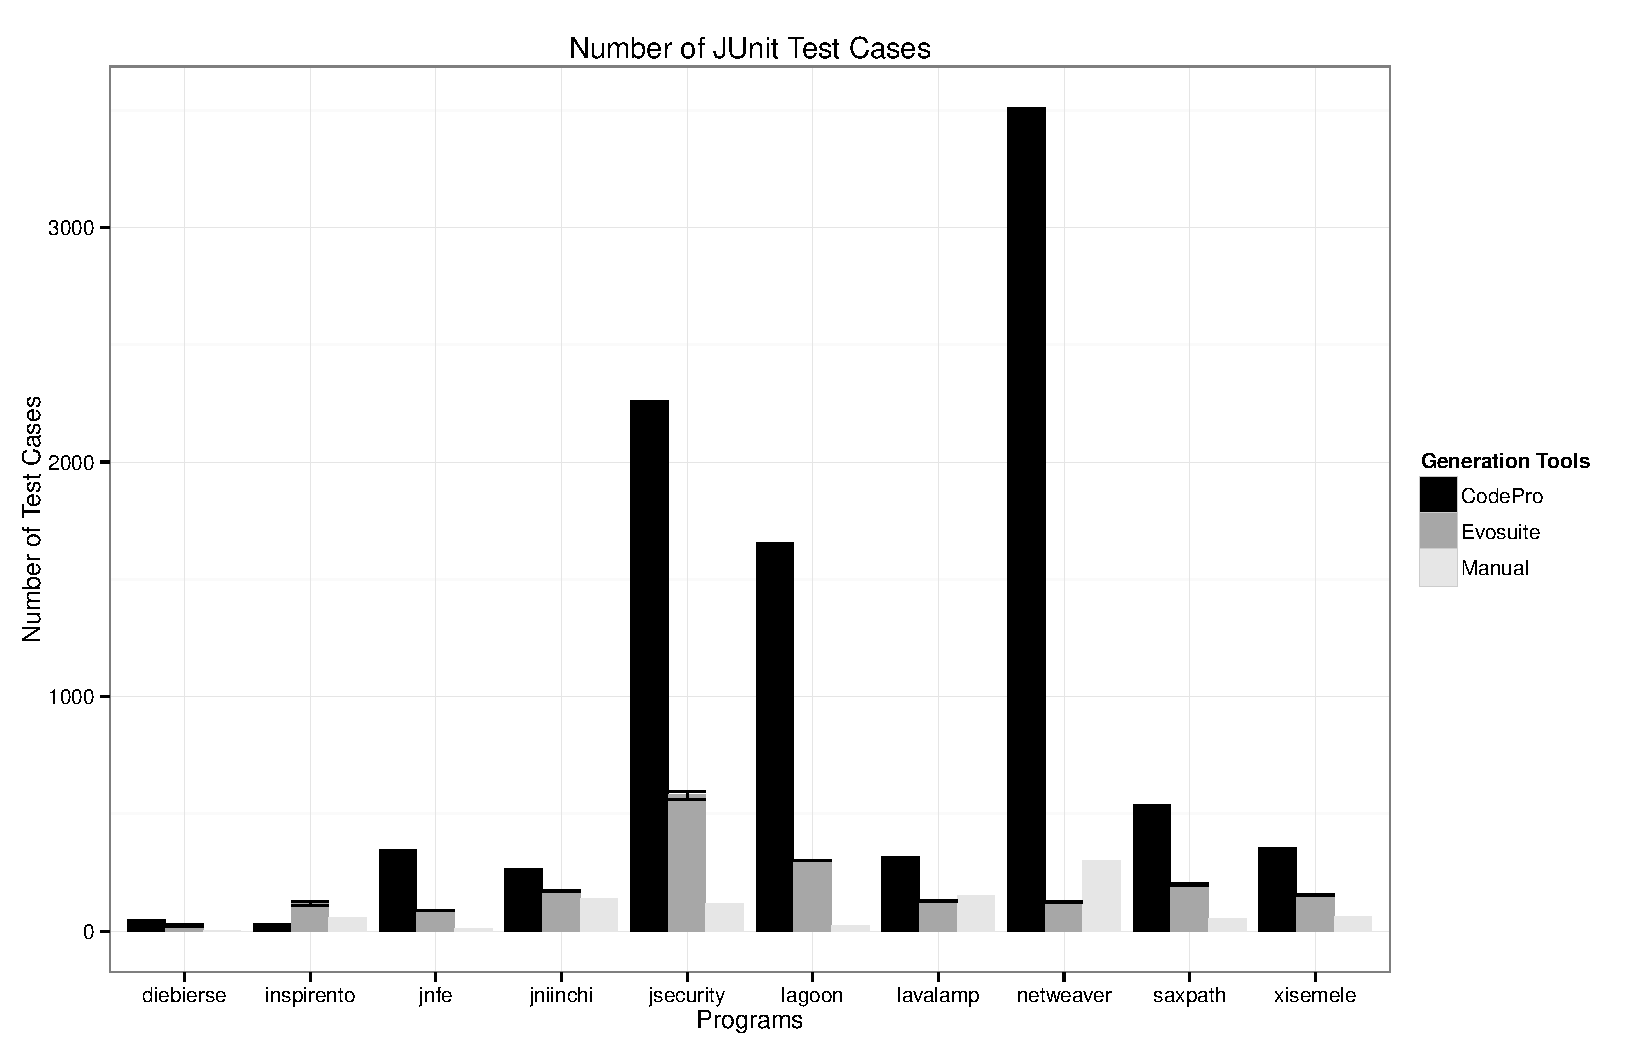
\includegraphics[scale=0.5]{RGraphs/TestCasesGenerated.pdf}
    \caption{Number of Test Cases per Test Suite.}
  \label{fig:NumTests}
\end{figure*}

After the case study applications were identified and analyzed, automated test tools \textsc{EvoSuite} and Codepro were used to generate test suites~\cite{CodePro1, fraser:2011:eat:2025113.2025179}. As \textsc{EvoSuite} is non-deterministic and learning-based, ten sets of tests were generated for evaluation, and the standard deviation is given across the ten test generations for all \textsc{EvoSuite} related results.  \textsc{EvoSuite} was configured using its default values~\cite{arcuri2013}.

\noindent \textbf{Evaluation Metrics:}

The manually written test suites and automatically generated test suites are compared based upon the time to generate test suites, the number of test cases generated, the time to execute generated tests, lines of code in the benchmark application, complexity of the benchmark application, branch coverage of generated suites, and the mutation score of generated suites. To perform these evaluations, three tools are used.

All tests are written or generated in JUnit form.  The time to generate test cases, number of test cases generated, and the time to execute the test suite are measured using the JUnit tool.  We also measure the non-commented LOC from the source code of the benchmark applications through JavaNCSS~\cite{leejavancss}.  

Following the automatic generation of test cases, Jacoco~\cite{jacoco} is used to calculate branch coverage of the tests.  Jacoco calculates branch coverage by instrumenting all branches at the byte code level through ASM, an all purpose Java bytecode manipulation and analysis framework. We also use MAJOR~\cite{just2011} to calculate fault-based mutation scores given the case study and associated tests. MAJOR is a Java compiler-integrated mutator that serves as a mutation analysis back-end for JUnit tests.  It provides a domain specific language to configure the mutation process, although we used its default values for our experiments.

\subsection{Experiments and Results}
Experiments were run to compare how test suites are generated using automated tools, the differences between the resulting test suites in terms of size and complexity, and the over all quality of the generated test suites.  

\subsubsection{Generating Test Suites }
%Time to generate
In the first set of experiments, we tracked the time required to generate the test suites, the number of test cases generated, and the execution time of the resulting test suite.  Figure~\ref{fig:TimeGen} displays the time required to generate each test suite using the two automatic test case generation tools, CodePro and \textsc{EvoSuite}.  In the case of Netweaver, CodePro completed test suite generation in approximately 51 minutes whereas \textsc{EvoSuite} required 89 minutes.  This was a small difference of 1.7\% compared to Xisemele, for which CodePro generated a test suite in just 13 seconds compared to 32 minutes from \textsc{EvoSuite}.  The time needed by \textsc{EvoSuite} was 148\% greater in this case.  On average, \textsc{EvoSuite} took 78\% more time in test generation compared to CodePro.

%# of tests
Next, the number of test cases generated per method was analyzed.  Figure~\ref{fig:NumTests} shows the number of tests generated.  For the ten case study applications, CodePro produced an average of  5\% more test cases than \textsc{EvoSuite} and 16.4 \% more than were written manually.  \textsc{EvoSuite} produced, on average, 4\% than were created manually. 

%Execution time
The time to execute the generated test suites was also evaluated. Figure~\ref{fig:TestExecTime} reveals that the execution time between manual, \textsc{EvoSuite}, and CodePro test suites, with test execution times ranging from between 2.1 to 25.5 seconds. In comparison to Figure~\ref{fig:NumTests}, the netweaver test suite contains the the most test cases. However, the netweaver CodePro test suite does not take the longest to execute.  Rather, the second largest test suite, jsecurity by \textsc{EvoSuite}, does. This may be the result of skeleton-like test cases that CodePro produces. CodePro's skeleton-like test cases provide comments for developers to find where to write test cases, forming a hybrid approach to the automated and manual world of testing.%\footnote{ For more information on the composition of these test cases, please reference our material at this web page: http://cs.uccs.edu/~kjustice/QSIC2014/} 

%Time of Execution
\begin{figure*}[!t]
\centering
  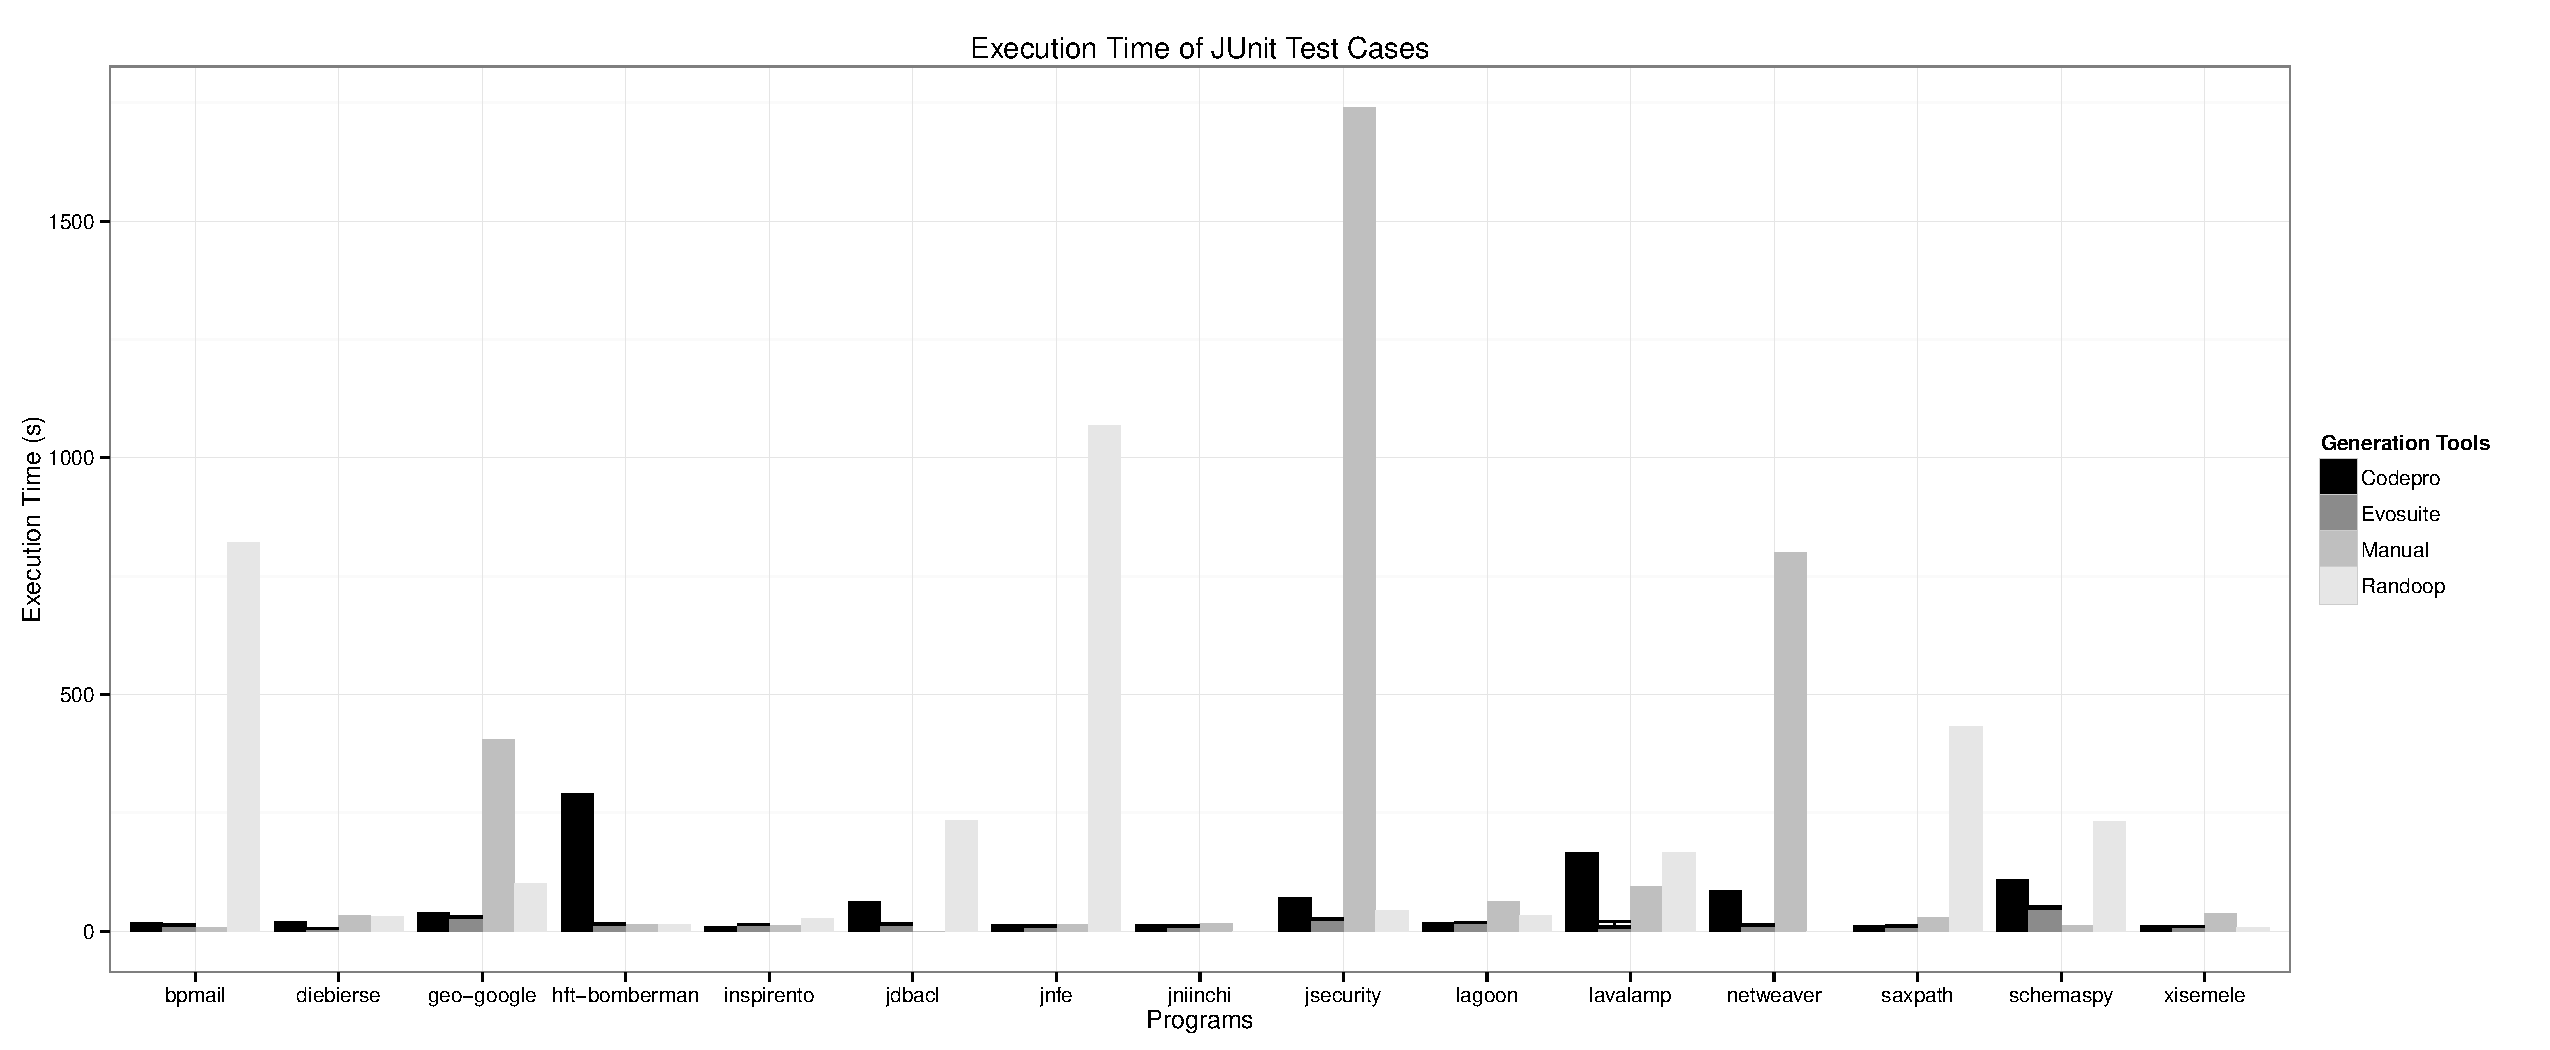
\includegraphics[scale=0.5]{RGraphs/TestExecutionTime.pdf}
    \caption{Execution Time of all Test Suites.}
  \label{fig:TestExecTime}
\end{figure*}

\subsubsection{Comparing Generated Tests to Case Studies}
%Number of Tests Versus LOC%
%CodPro and and Evosuite retain high $R^2$ values averaging at PERCENT . As the lines of code increases, the number of generated test cases increases. CodePro had by far the most generated test cases and lines of code, averaging over PERCENT more test cases than either Evosuite or the manually written test suites. Evosuite averaged PERCENT more test cases than manual tests. Manual test suites contained the least amount of lines of code and written tests. The overall trend between the LOC and number of test cases for manual were positive, but did not correlate as strongly as the automated test suites did.

%Time to Generate vs Complexity%
%CodePro takes much less time than Evosuite to generate the test suite. Evosuite test generation took PERCENT amount of time longer. Both graphs indicated that more complex applications require longer times to generate test suite. 


%LOC
The LOC for the generated test suites and the application source code were also compared. Figure~\ref{fig:LOC} shows that CodePro generates more LOC than either manual or \textsc{EvoSuite} test suites. As shown in Figure ~\ref{fig:NumTests}, CodePro generated the most tests out of the automated test generators. In a comparison between the two graphs, the a close correlation can be seen between the LOC and the number of tests. For example, netweaver contains 17953 LOC, and CodePro produces 3513 test cases for the application. Likewise, the other applications and their tests suites share this same trend. As the size of the application increases, the number of tests will increase as well. In proportion to the original lines of code, the number of test cases are greatest with CodePro, then \textsc{EvoSuite}, and then manual. 
 
%Branch Cov
%Mutation Score



%LOC (source)
\begin{figure*}[!t]
\centering
  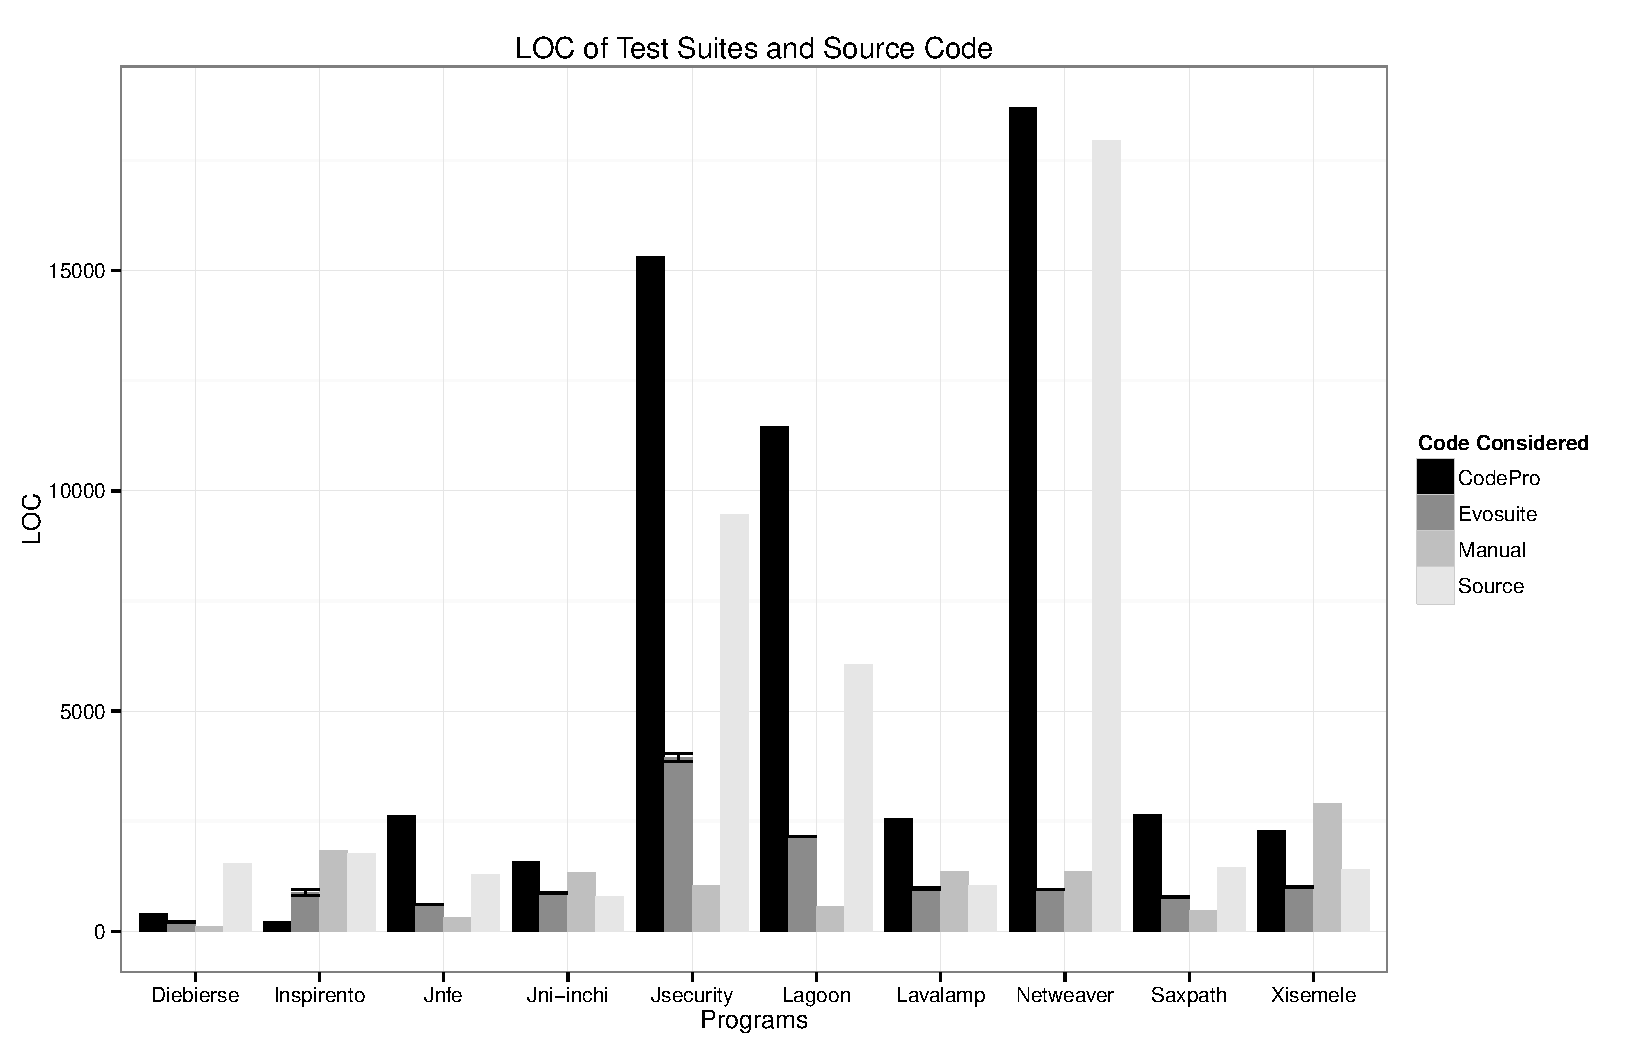
\includegraphics[scale=0.5]{RGraphs/LOC.pdf}
    \caption{Non-commented lines of code for automatically generated tests and manual tests compared to case study source code. }
  \label{fig:LOC}
\end{figure*}
%Complexity (source)-- do we really compare about complexity of tests versus complexity of source? Leaving out.


\subsubsection{Quality: Manual versus Generated}
In this study, both branch coverage and mutation scores were measured for each of the generation test suites. The branch coverage for manually test suites varied greatly, but was the only method  able to attain a score over 70\% with Lavalamp and Xisemele. Both applications contained the least number of test cases with manual as evidenced by  Figure~\ref{fig:NumTests}. Overall CodePro had higher branch coverage scores than \textsc{EvoSuite} or manual. This could indicate a direct relationship between the number of tests and the branch coverage. 

%Number of Tests vs Branch Coverage%
The relationship between the number of tests and the branch coverage for each test generated suite was furthermore examined. In comparing Figure~\ref{fig:NumTests} and the branch coverage, manual test suites increased in branch coverage as the number of test cases increased. When evaluating \textsc{EvoSuite}, the trend line has a low  $R^2$ value at 0.184, but begins in a similar trend to manual and CodePro, and actually drops in branch coverage for the two larger test suites. The branch coverage in comparison with the number of tests indicates that CodePro branch coverage drops as the number of generated test cases increases. Larger, more complex applications may require more tests to be written to increase the branch coverage. 

%\begin{figure}[!t]
%\centering
 % 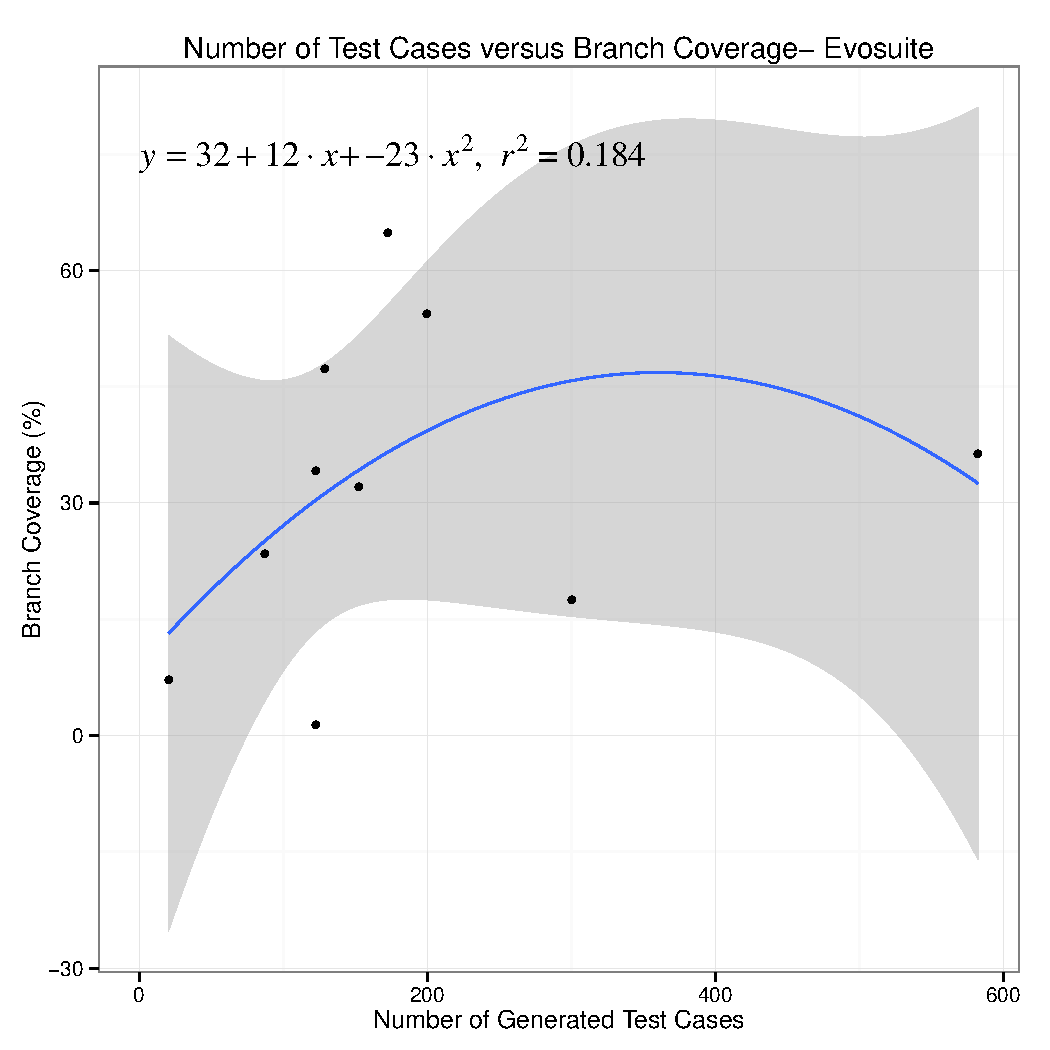
\includegraphics[width=\linewidth]{RGraphs/Evosuite_TestsVersusBranchCov_poly.pdf}
 %   \caption{Number of tests compared to the branch coverage of Evosuite.}
 % \label{fig:NumTestsvsBranchCov}
%\end{figure}

%LOC vs Branch Coverage%	
Our next experiment evaluates the relationship between LOC and Branch coverage for each of the generated test suites.  \textsc{EvoSuite}, CodePro, and manual test suites demonstrated a similar trend in the decrease of Branch Coverage as the LOC of the application code increased. Only CodePro displays a larger increase in branch coverage by at least 27\%  more for the largest program, netweaver, in comparison with  \textsc{EvoSuite} and manual. Despite generating more tests in proportion to the application source code size,  CodePro did not meet the quality of the tests generated by \textsc{EvoSuite} or the manually written test suites.

\begin{figure}[!t]
\centering
  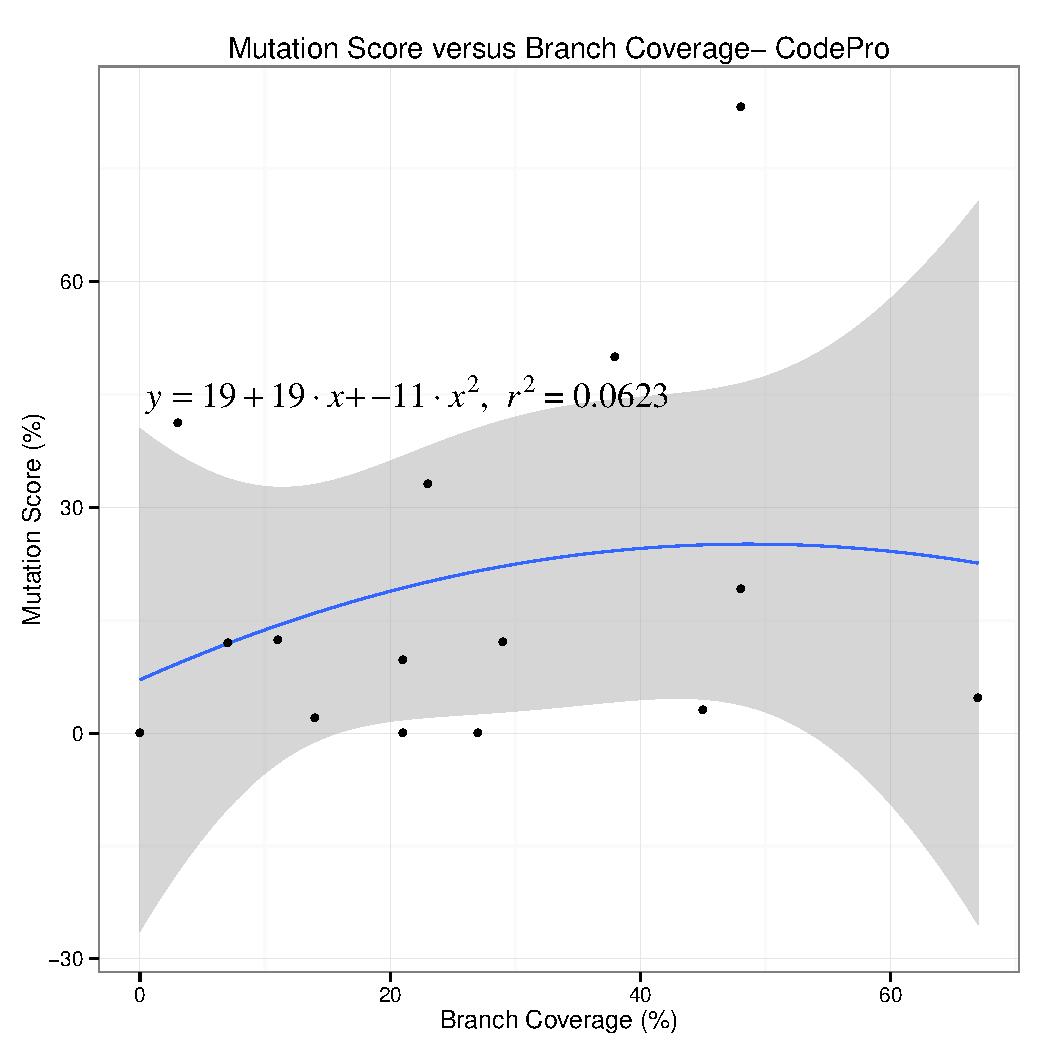
\includegraphics[width=\linewidth]{RGraphs/CodePro_BranchCov_versus_Mutation_poly.pdf}
    \caption{Mutation Score compared to Branch Coverage for test suites generated by CodePro.}
  \label{fig:CP_branch_mutation}
\end{figure}
%Mutation score%
For the mutation score, \textsc{EvoSuite} attained the highest scores for five of ten applications. However, dieberse scores ranged dramatically between 18\% and 40\%.  CodePro resulted in the worst mutation scores, acquiring a  0\% mutation score for lagoon, saxpath, and xisemele. This is due to the skeleton-like tests that CodePro often creates.  While these tests can lead to the execution of branching behavior due to the tool's goal of generating test cases that exercise each line of code, the oracles, if they exist, are often poorer than \textsc{EvoSuite}'s intelligent oracles and thus miss capturing faults. \textsc{EvoSuite}, on the other hand, was able to generate test suites averaging between 33.7\% and 77.1\% for these applications. Manual tests remained between 18.3\% and 56.5\%  mutation scores between the applications, while CodePro's mutation scores ranged between 0\% and 41.3\%. 

%Branch Coverage vs Mutation%
% ~\ref{fig:manual_branch_mutation},~\ref{fig:Evo_branch_mutation}, and ~\ref{fig:CP_branch_mutation} compares the

Figures~\ref{fig:CP_branch_mutation},~\ref{fig:Evo_branch_mutation}, and~\ref{fig:manual_branch_mutation} compare the branch and mutation score for manually generated test suites, \textsc{EvoSuite}'s test suites, and CodePro-generated suites, respectively.  In general, the mutation score increased as the branch coverage increased.  Figure~\ref{fig:CP_branch_mutation} displays a much lower $R^2$ value at 0.137, but the data indicates overall that the mutation score neither increases nor decreases with higher branch coverage. This can be explained because the mutation scores were all much lower than manual and \textsc{EvoSuite} scores. With exception to the outlier of a 40\% mutation score, the trend would otherwise indicate that the mutation score increases as the branch coverage increases.

  For each comparison, the Kendall $\tau$ coefficient and Pearson's product-moment correlation were calculated.  While there is a possibility of rank ties when calculating Kendall's $\tau$ values, none were identified in this work.  In comparing the coverage and mutation scores for CodePro, Kendall $\tau$'s coefficient is -0.0698.  The Pearson's test gives a correlation of -0.275. 
For ~\textsc{EvoSuite}, the Kendall $\tau$'s coefficient is 0.111.  The Pearson's test gives an overall correlation value of 0.212.  
Manually written tests earn a Kendall $\tau$ value of 0.135.  The Pearson's test reveals an overall correlation of 0.155.  

The Kendall $\tau$ measurement of correlation, calculated in {\tt R}, falls between -1 and 1, representing a strong negative and strong positive association, respectively, and with 0 showing no correlation. We use an accepted interpretation of $\tau$, whereby the qualitative terms ``small'', ``medium'' and ``large'' correspond to 0.1, 0.3 and 0.5~\cite{kraemer2003}.  For CodePro, there is essentially no correlation between branch coverage and mutation scores.  \textsc{EvoSuite} demonstrates a small correlation, and manually written tests have a slightly larger, but still small, correlation. 

\begin{figure}[!t]
\centering
  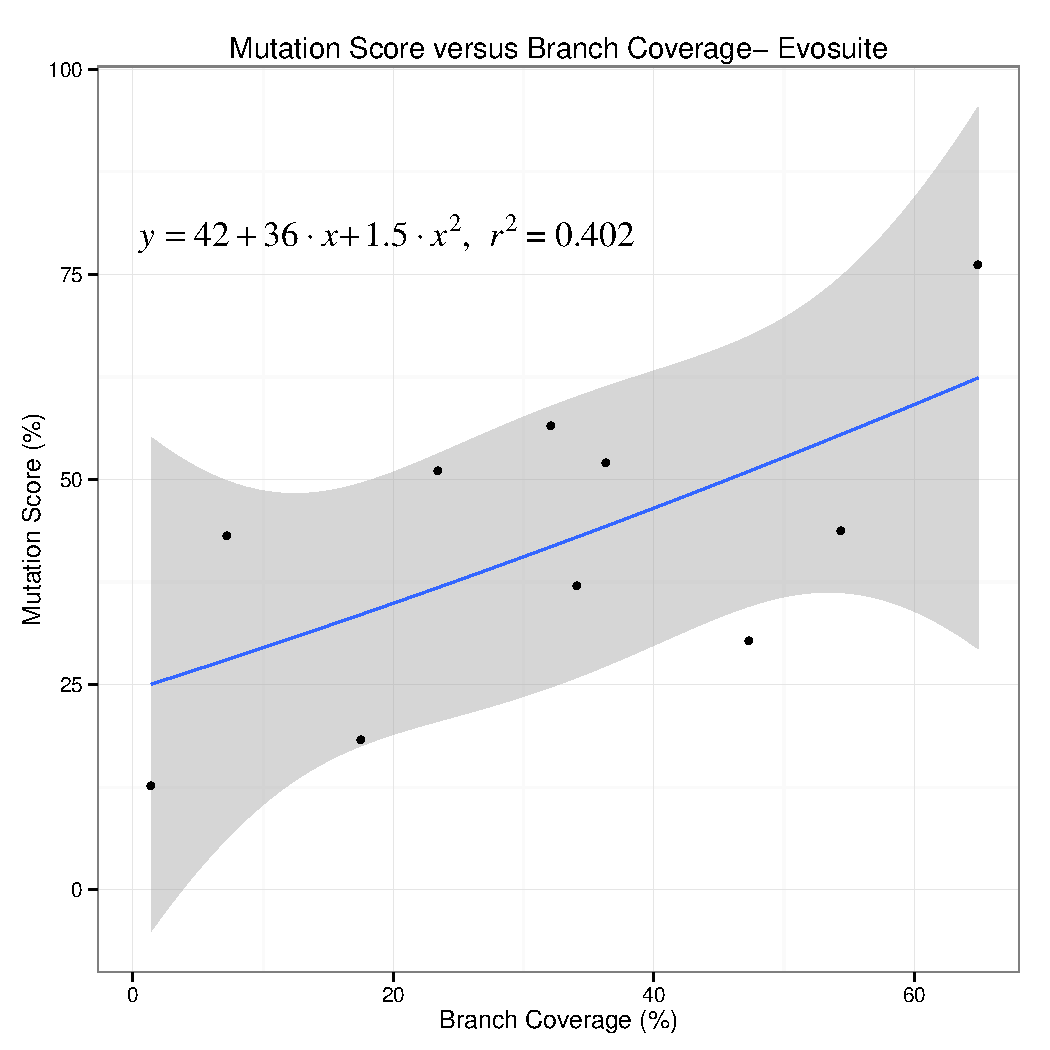
\includegraphics[width=\linewidth]{RGraphs/Evosuite_BranchCov_versus_Mutation_poly.pdf}
    \caption{Mutation Score compared to Branch Coverage for test suites generated by Evosuite.}
  \label{fig:Evo_branch_mutation}
\end{figure}
\begin{figure}[!t]
\centering
  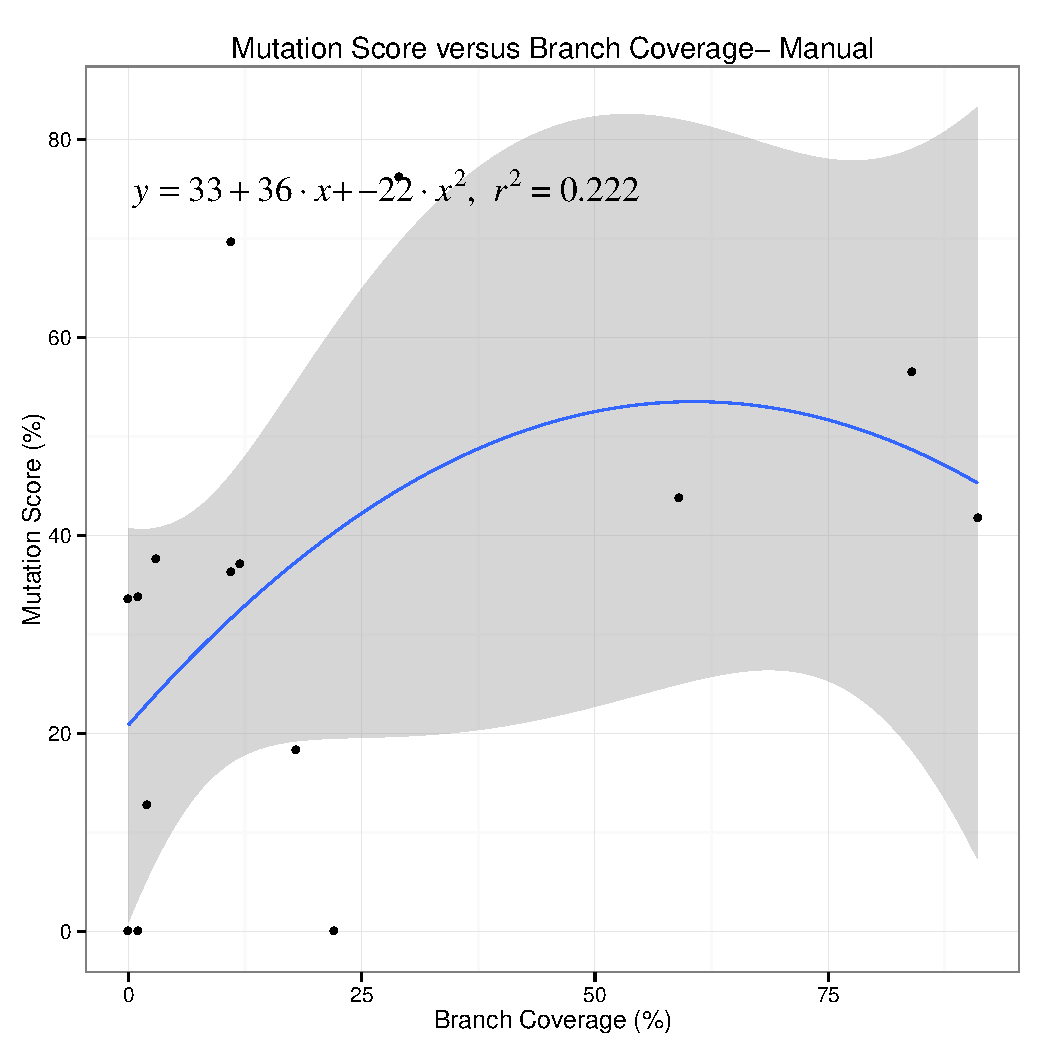
\includegraphics[width=\linewidth]{RGraphs/Manual_BranchCov_versus_Mutation_poly.pdf}
    \caption{Mutation Score compared to Branch Coverage for test suites created manually.}
  \label{fig:manual_branch_mutation}
\end{figure}

The Pearson's product-moment correlation is similarly between -1 and 1.  A value of 1 implies that a linear equation
describes the relationship between X and Y perfectly, with all data points lying on a line for which Y increases as X
increases.  A value of -1 implies that all data points lie on a line for which Y decreases as X increases. A value of 0
implies that there is no linear correlation between the variables. The results between the Kendall $\tau$ and Pearson's
correlations agree for all three sets of data.  While correlations do exist between the branch coverage and mutation
scores for \textsc{EvoSuite} and manually written tests, they are small.  The correlation between the branch coverage
and mutation scores of CodePro are slightly negative.  


%Complexity vs Mutation%
%We further examined the relationship between the Cyclomatic Complexity of the application source code and the mutation score of the generated test suite. For manual test suites, Figure MANUAL indicates that applications with a higher complexity received lower mutation scores. Figure EVOSUITE shows that the two most complex programs that manual test suites received the lowest mutation scores for received just about the same scores as less complex applications with Evosuite. Less complex applications received overall higher mutation scores with Evosuite. Figure CODEPRO reveals that the most and least complex programs both received mutation scores of 0. Regardless of complexity, all of the mutation scores are low for CodePro.

%More info%
For full result analyses including full Kendall $\tau$ analyses and Pearson correlation summaries, in addition to more
results and graphs from our evaluations related to LOC of the generated test suites, cyclomatic complexity of the test
suites, and cyclomatic complexity of the application source code, please refer to: \url{http://cs.uccs.edu/~kjustice/QSIC2014/.}

\subsection{Threats to Validity}
%\noindent \textbf{Internal Validity}

There are several threats to the validity of this work.  First, \textsc{EvoSuite} was used to generate test suites using its default configuration values. While tuning can have impact on the performance of a search algorithm, in the context of test data generation, it is difficult to find good settings that significantly outperform the ``default'' values suggested in the literature~\cite{arcuri2013}.  Thus, the default values were used.  Presented results in this paper represent ten test suites generated by \textsc{EvoSuite}.  Although more test suites were generated for a subset of the applications, the average and standard deviation remained the same given more executions of \textsc{EvoSuite}, and thus, ten generated test suites can be viewed as sufficient.

Second, the determination of the quality of software tests can be considered a subjective measurement. Although mutation score and coverage are two ways to measure test suite quality, that does not consider the readability of the test cases.  If the developers who need to view tests in order to diagnose defects cannot understand what the tests do, then the human time and effort could be substantially increased.

Third, the tools used for coverage and mutation analysis also lead to a potential internal threat to validity.  Jacoco was used for all coverage analysis, and MAJOR was used for mutation analysis.  Jacoco, a well-established coverage monitor for Java programs, is based on Emma, another standard tool for analyzing Java programs~\cite{jacoco}.  MAJOR~\cite{just2011} is an experimentally verified (e.g., \cite{just2014}) and well tested (e.g., \cite{just2011b}) mutation testing tool integrated into the Java compiler. However, other options such as PIT~\cite{ pit2014} could be used in future comparisons. 

%The statistical analysis also may be a threat to validity, as the inconsistency in how both \textsc{EvoSuite} and manually written tests are created. Also, CodePro generated some test suites with a mutation score of 0, which could mislead one to believing that CodePro has no use for creating quality tests. For this reason we removed these results to give a better impression of the trend CodePro test suites.

%\noindent \textbf{External Validity}

%\noindent \textbf{Construct Validity}
\section{Discussion}
\label{sec:discussion}

In comparing LOC and number of test cases, we observe that higher proportions of test cases compared to original application code does not necessarily imply that either mutation score or branch coverage will be high.  Especially in the case of CodePro, in which many tests are produced in a skeleton-like fashion, the mutation scores and branch coverage are much lower than  \textsc{EvoSuite} and manual tests. However, as indicated earlier, the skeleton approach to generation gives developers a template to easily modify and implement. Automated test suite generation can aide the developer in covering a large portion of the application, allowing developers to reduce the time and effort spent in identifying source code to be covered by tests and then enhancing the tests later.  Although this feature could be desirable for developers who want help in achieving high coverage, it will still require more manual effort than fully automated test generation tools such as \textsc{EvoSuite}.

As seen from the results, learning-based test suite generation tools are more helpful in creating executable test cases that do not need modification prior to use.  These tests attain coverage and mutation scores that are only slightly lower than manually written test suites.  On average, the branch coverage scores are comparable, and mutation scores are only about 1\% less than manual tests.  However, the modifiability and readability of the resulting tests varies.  For example, CodePro tends to create tests that build empty object-oriented tests that are executable, but require the developer to generate complete test oracles.  Thus, CodePro's mutation scores especially are lower than those written by a human or through a learning-based tool.  \textsc{EvoSuite}, on the other hand, creates more complete tests.  \textsc{EvoSuite} will additionally write tests focusing on exceptions, and parameter paths.  As \textsc{EvoSuite} takes potential faults into consideration as it ``grows'' tests, its mutation scores are higher.  Manual tests are generally written with the functionality of the program itself in mind.  While all three processes have their benefits, the learning capability of tools like \textsc{EvoSuite} to achieve high-quality results in little time gives a strong initial set of tests that can then be broadened as developers enhance their knowledge of the code under test.

%From a pure comparison of quality between \textsc{EvoSuite}, CodePro, and manually written test suites, manual test suites have the potential for attaining the highest coverage and mutation scores. Potential can only be measured by the individual writer of the tests, and could be one of the reasons the data relating to the manual test suites are less consistent than that of \textsc{EvoSuite} and CodePro. \textsc{EvoSuite} almost retains the same quality as Manual tests, achieving an average of only one percent less in total for mutation score of \textsc{EvoSuite} at 39.8\%  and manual with 40.3\%. \textsc{EvoSuite} would reduce the time and cost of implementing the tests in comparison to manual tests. Also \textsc{EvoSuite} can maintain the relative quality as manual tests, but provide little modifiability of the tests, as the genetic algorithm changes the test suite every time.
